\setcounter{chapter}{4}
\setcounter{section}{0}
\part{RESULTADOS Y DISCUSIÓN} 

\section{Resultados de la metodología}

Los resultados que se obtuvieron al aplicar la metodología basada en el manifiesto del desarrollo de software ágil se redactan a continuación:

\subsection{Análisis de requisitos y obtención de pruebas}

Para llevar a cabo el análisis de los requisitos sobre la librería JavaScript que se desarrolló se tomaron en cuenta varios favores observando las carencias que existen al momento de realizar el modelamiento de cualquier software. Mediante el docente encargado de impartir las clases sobre cómo utilizar los lenguajes de modelado como lo es UML se dio cuenta que podría existir una forma en generar uno de los diagramas más importantes que es el diagrama de clases, pero a partir de las descripciones que se generan en los casos de uso del sistema.

Existe una herramienta denominada TDDT4IoTS que permite realizar el modelamiento de varios tipos de software. La herramienta cuenta con un lenguaje de símbolos que permiten escribir dentro de las descripciones de casos de uso datos técnicos sobre los objetos que intervendrán en el sistema informático que llevara a cabo la ejecución de todos los escenarios que se están describiendo. A petición del cliente recomendó que visitemos el sitio web de aplicaciones.uteq.edu.ec/tddt4iots para visualizar  los símbolos que usa la herramienta (ver figura \ref{fig:simbolostdd}).

\begin{figure}[H]
	\caption{Símbolos que utiliza la herramienta TDDT4IoTS}
	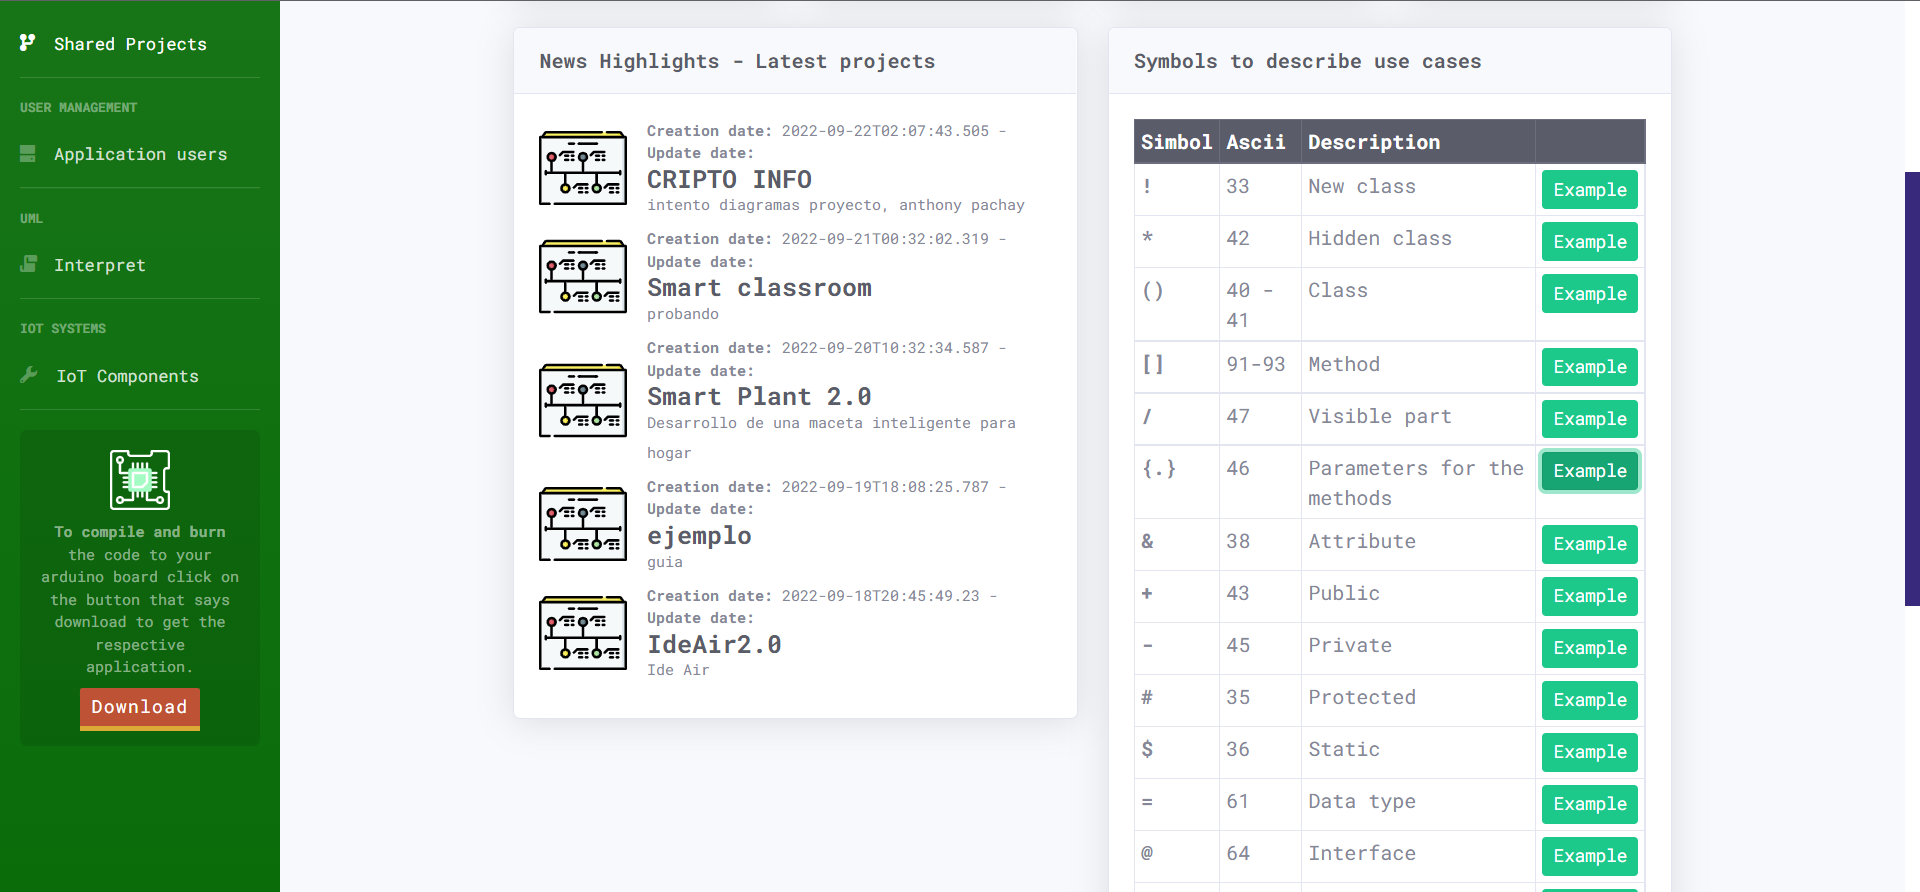
\includegraphics[width=14cm]{img/res_001.png}
	\label{fig:simbolostdd}
	\textbf{\\ FUENTE: PROPIA \\ ELABORADO: DÚVAL CARVAJAL SUÁREZ}
\end{figure}

En la lista de símbolos que se visualizar en la figura anterior se encuentra un botón que dice \textit{"Example"}. Si presionamos en ese botón se pudo observar un ejemplo detallado sobre como se deben utilizar los símbolos para tratar de especificar algún objeto del diagrama de clases que se generar mediante la descripción del caso de uso pertinente (ver figuras \ref{fig:ejemploclase}, \ref{fig:ejemploparametro}).

\begin{figure}[H]
	\caption{Ejemplo de como se debe utilizar el símbolo respectivo para crear una clase.}
	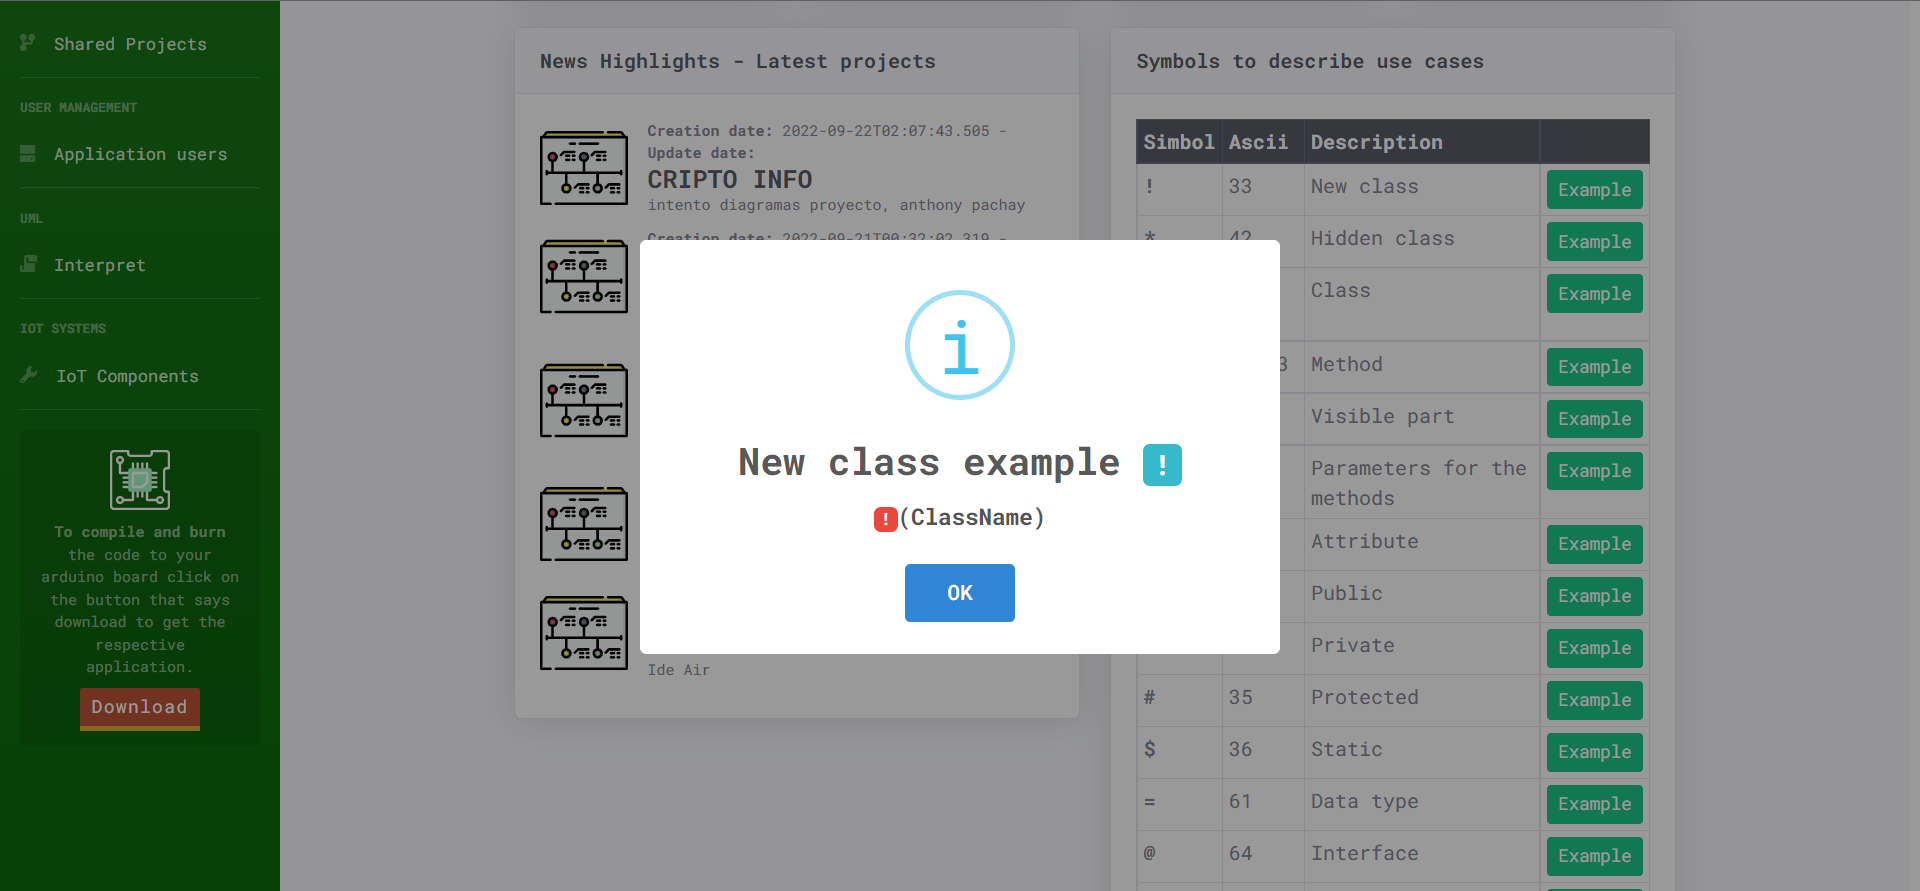
\includegraphics[width=14cm]{img/res_002.png}
	\label{fig:ejemploclase}
	\textbf{\\ FUENTE: PROPIA \\ ELABORADO: DÚVAL CARVAJAL SUÁREZ}
\end{figure}

\begin{figure}[H]
	\caption{Ejemplo de como se debe utilizar el símbolo respectivo generar los parámetros de un método declarado con el lenguaje de símbolos.}
	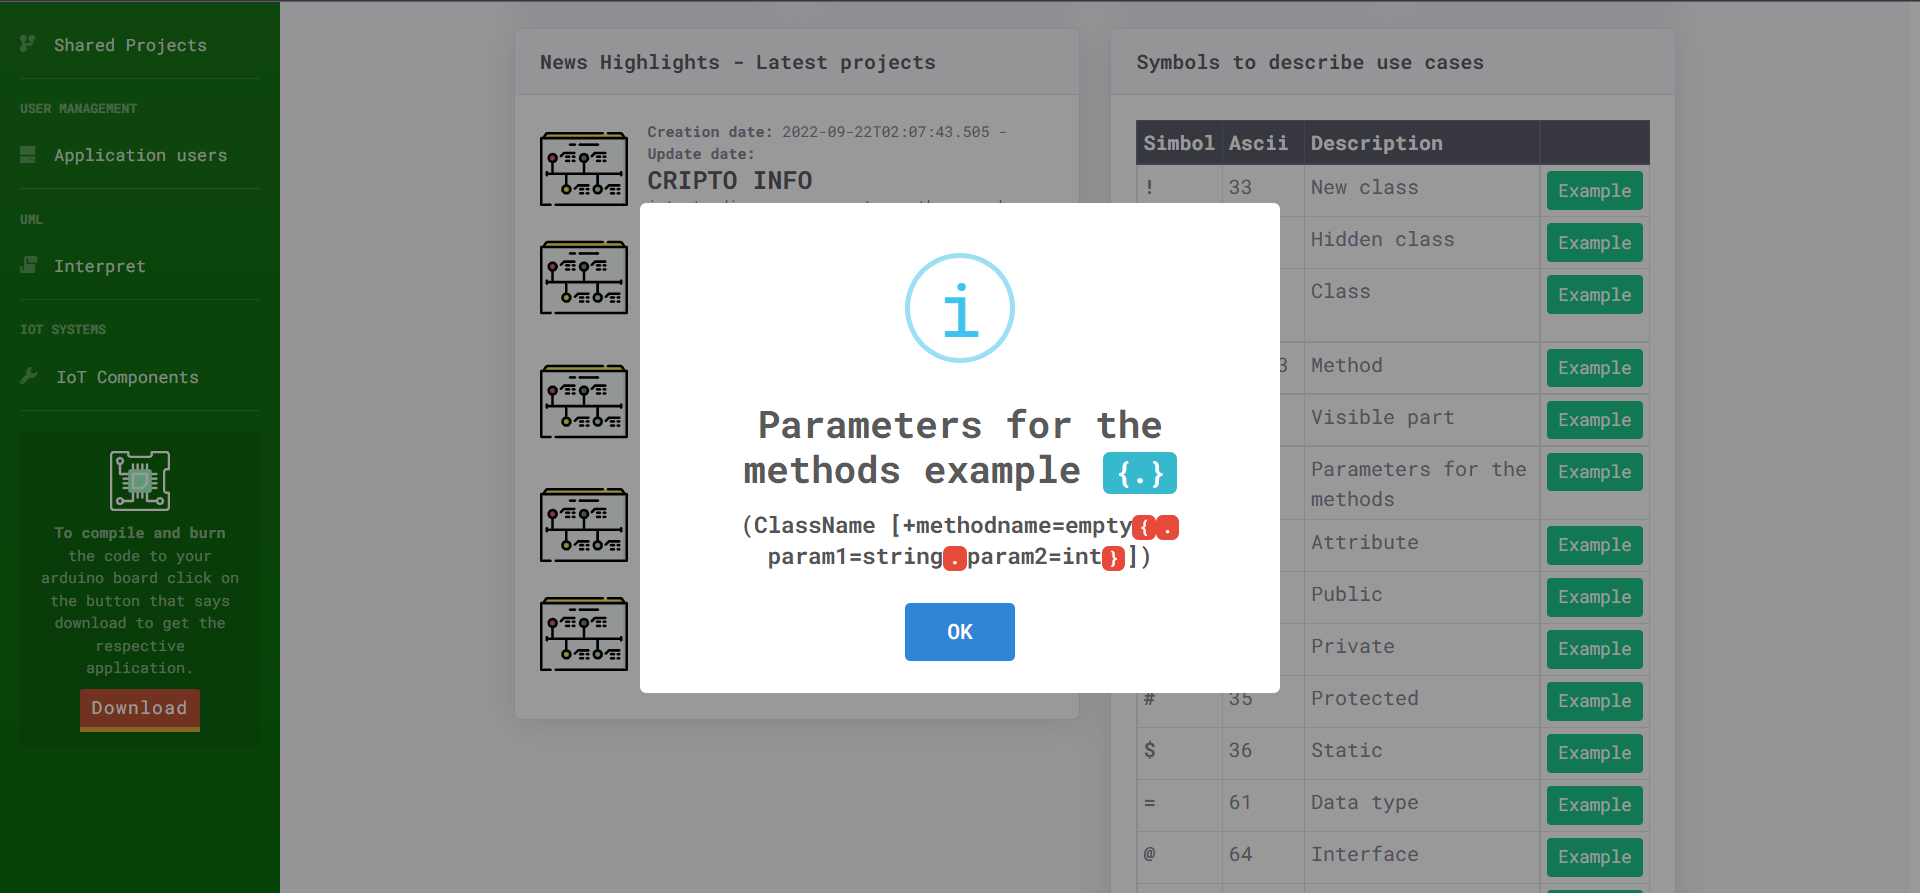
\includegraphics[width=14cm]{img/res_003.png}
	\label{fig:ejemploparametro}
	\textbf{\\ FUENTE: PROPIA \\ ELABORADO: DÚVAL CARVAJAL SUÁREZ}
\end{figure}

Luego de tener una idea general sobre los símbolos que utiliza la herramienta se especificaron detalladamente los significados de cada símbolo y como puede ser utilizado en las descripciones de los casos de uso.  

\begin{itemize}
	\item \textbf{Asterisco *}: Este símbolo sirve para ocultar cualquier carácter que se encuentre redactado después el. Esto permitirá al momento de interpretar la descripción del caso de uso ingresada eliminar los caracteres mezclados con los símbolos y solo dejar visibles los caracteres normales formando un texto natural que pueda ser entendido por cualquier persona regular. \textbf{Ejemplo:}
	
	\begin{verbatim}
		* texto de prueba
	\end{verbatim}
	
	\item \textbf{Paréntesis de apertura y cierre ()} : Este símbolo sirve para especificar uno de los componentes más importantes del diagrama de clases, dentro de los paréntesis de apertura y cierra se deberá especificar el nombre de la clase u objeto que se pretende generar de forma automática. Cabe mencionar que, si se escribe el nombre de clase separada por espacios, la librería deberá omitir estos espacios y auto completarlos con la segunda letra después del espacio con mayúscula. \textbf{Ejemplo:}  
	
	\begin{verbatim}
		(Nombre de la clase)
	\end{verbatim}
	
	\item \textbf{Corchete de apertura y cierre []:} Este símbolo podrá ser utilizado dentro de los símbolos para crear las clases, permitirá definir Los métodos o funciones que pertenecerá a la clase respectiva. \textbf{Ejemplo:} 
	
	\begin{verbatim}
		(Nombre de la clase [+nombre del metodo=empty])
	\end{verbatim} 
	
	\item \textbf{Slash /:} Este símbolo es bastante interesante, con el se debe visualizar cualquier caracteres que se encuentre encerrado de un slash de apertura y otro slash de cierre. Este símbolo se lo deberá usar cuando todos los caracteres se encuentren después del símbolo del asterisco, la idea es permitir que se visualicen caracteres específicos dentro de los datos técnicos para generar el diagrama de clases, sin afectar el uso de los demás símbolos. \textbf{Ejemplo:}
	
	\begin{verbatim}
		(Nombre de la clase &+/nombre/=string)
	\end{verbatim} 
	
	\item \textbf{Llaves de apertura y llaves de cierre con punto \{.\}:} Con el símbolo de las llaves se podrá definir los parámetros de entrada para los métodos o funciones de las clases. Cada parámetro estará separado por un punto, además se deberá utilizar el símbolo del igual (=) para especificar su tipo de dato. Cada recalcar que todos los atributos también deberán estar especificados dentro de las llaves de apertura y cierre. \textbf{Ejemplo:}
	
	\begin{verbatim}
		(Nombre de la clase [+nombre del metodo=empty
		{.param1=string.param2=strgin}])
	\end{verbatim}
	
	\item \textbf{Ampersand \&: } Este símbolo debe permitir declarar los atributos de la clase que fue creada con el símbolo anterior. Existen otros símbolos que interviene en la creación de otros componentes del diagrama de clases, más adelante se detallaran para que sirven. \textbf{Ejemplo:}
	
	\begin{verbatim}
		(Nombre de la clase &+atributo uno=string &+atributo 
		dos=string)
	\end{verbatim}
	
	\item \textbf{Visibilidad +: } El símbolo de suma permite especificar que la visibilidad del atributo, método o función será de manera pública. \textbf{Ejemplo:}
	
	En este ejemplo se visualiza la forma en cómo utilizar el símbolo de suma en atributos de clase.
	
	\begin{verbatim}
		(Nombre de la clase &+atributo uno=string &+atributo 
		dos=string)
	\end{verbatim}
	
	En este ejemplo se visualiza la forma en cómo utilizar el símbolo de suma en métodos o funciones de clase.
	
	\begin{verbatim}
		(Nombre de la clase [+nombre del metodo=empty
		{.param1=string.param2=strgin}])
	\end{verbatim}
	
	\item \textbf{Visibilidad -: } El símbolo de resta permite especificar que la visibilidad del atributo, método o función será de manera privada. \textbf{Ejemplo:}
	
	En este ejemplo se visualiza la forma en cómo utilizar el símbolo de suma en atributos de clase.
	
	\begin{verbatim}
		(Nombre de la clase &-atributo uno=string &-atributo 
		dos=string)
	\end{verbatim}
	
	En este ejemplo se visualiza la forma en cómo utilizar el símbolo de suma en métodos o funciones de clase.
	
	\begin{verbatim}
		(Nombre de la clase [-nombre del metodo=empty
		{.param1=string.param2=strgin}])
	\end{verbatim}
	
	\item \textbf{Visibilidad \#: } El símbolo de almohadilla permite especificar que la visibilidad del atributo, método o función será de manera protegida. \textbf{Ejemplo:}
	
	En este ejemplo se visualiza la forma en cómo utilizar el símbolo de suma en atributos de clase.
	
	\begin{verbatim}
		(Nombre de la clase &#atributo uno=string &#atributo 
		dos=string)
	\end{verbatim}
	
	En este ejemplo se visualiza la forma en cómo utilizar el símbolo de suma en métodos o funciones de clase.
	
	\begin{verbatim}
		(Nombre de la clase [#nombre del metodo=empty
		{.param1=string.param2=strgin}])
	\end{verbatim}
	
	\item \textbf{Visibilidad \$: } El símbolo de dólar permite especificar que la visibilidad del atributo, método o función será de manera estática. \textbf{Ejemplo:}
	
	En este ejemplo se visualiza la forma en cómo utilizar el símbolo de suma en atributos de clase.
	
	\begin{verbatim}
		(Nombre de la clase &$atributo uno=string &$atributo 
		dos=string)
	\end{verbatim}
	
	En este ejemplo se visualiza la forma en cómo utilizar el símbolo de suma en métodos o funciones de clase.
	
	\begin{verbatim}
		(Nombre de la clase [$nombre del metodo=empty
		{.param1=string.param2=strgin}])
	\end{verbatim}
	
	\item \textbf{Igual =:} El símbolo de igual debe permitir asignar el tipo de dato a los atributos, métodos o funciones declaradas dentro de la clase. En el caso de los métodos de tipo \textbf{void}  se deberá utilizar la palabra \textit{empty} indiciando que es un método que retornara ningún valor. \textbf{Ejemplo:}
	  
\end{itemize}

\section{Modelamiento}

Se utilizo el lenguaje de programación JavaScript con la intención de generar un paquete totalmente exportable a otros proyectos que requieran utilizar la librería para generar sus propios diagramas con otras librerías de dibujo. Para empezar con el diseño o modelamiento de la librería se especificó el proceso normal que deberá seguir la al momento de recibir como datos de entrada las descripciones de los casos de uso. En la figura \ref{fig:armadillocasodeuso} se observa el proceso que se llevara a cabo de forma general la ejecución de la librería.

En la figura \ref{fig:armadillocasodeuso} se pude observar el diagrama de casos de uso que explica las acciones que el analista podrá realizar al momento de implementar la librería, o podrá utilizar la aplicación de demostración


\begin{figure}[h!]
	\caption{Diagrama de casos de uso armadillo.}
	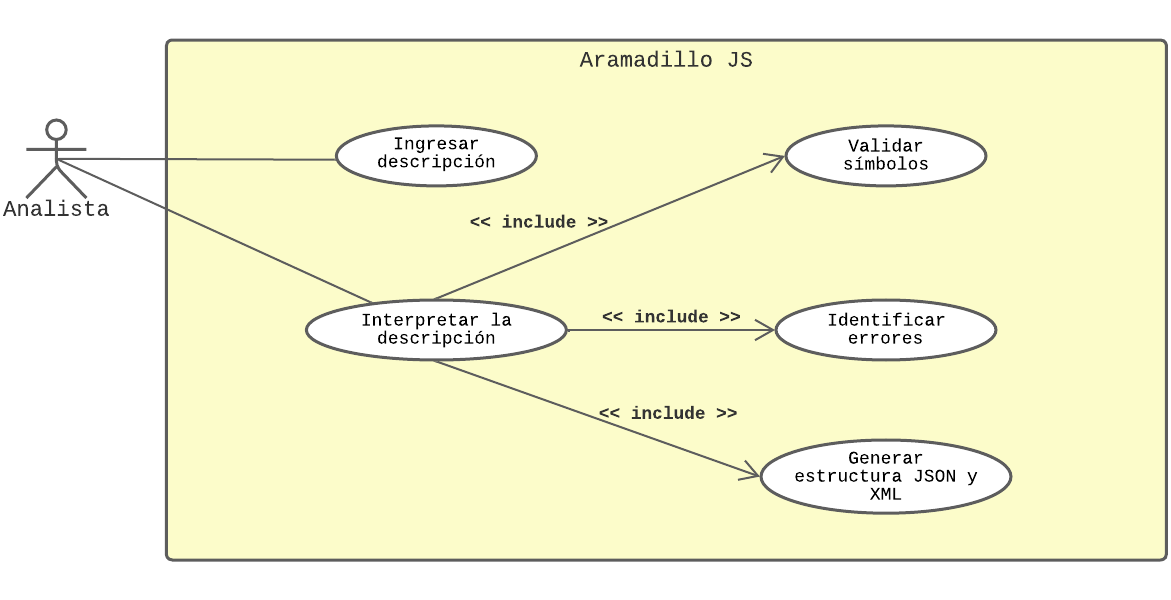
\includegraphics[width=15cm]{img/modelamientocasodeuso.png}
	\label{fig:armadillocasodeuso}
	\textbf{\\ \\ ELABORADO: DÚVAL CARVAJAL SUÁREZ}
\end{figure} 

A continuación, se detallarán las descripciones de los casos de uso que se utilizaron para la creación del diagrama.

Para cumplir con los requisitos recopilados en la fase anterior se realizaron diagramas de flujo para realizar el análisis pertinente a lo que la librería debe cumplir. Esto permitirá identificar las posibles fallas que se mostrarían al momento de estar utilizando la librería. En la figura \ref{fig:algoritmoerror} se observa el algoritmo que permitió identificar los errores en la escritura de las descripciones de los casos de uso utilizando el lenguaje de símbolos.


\begin{figure}[h!]
	\caption{Diagrama de flujo para detectar errores en las descripciones de los casos de uso utilizando un el lenguaje de símbolos.}
	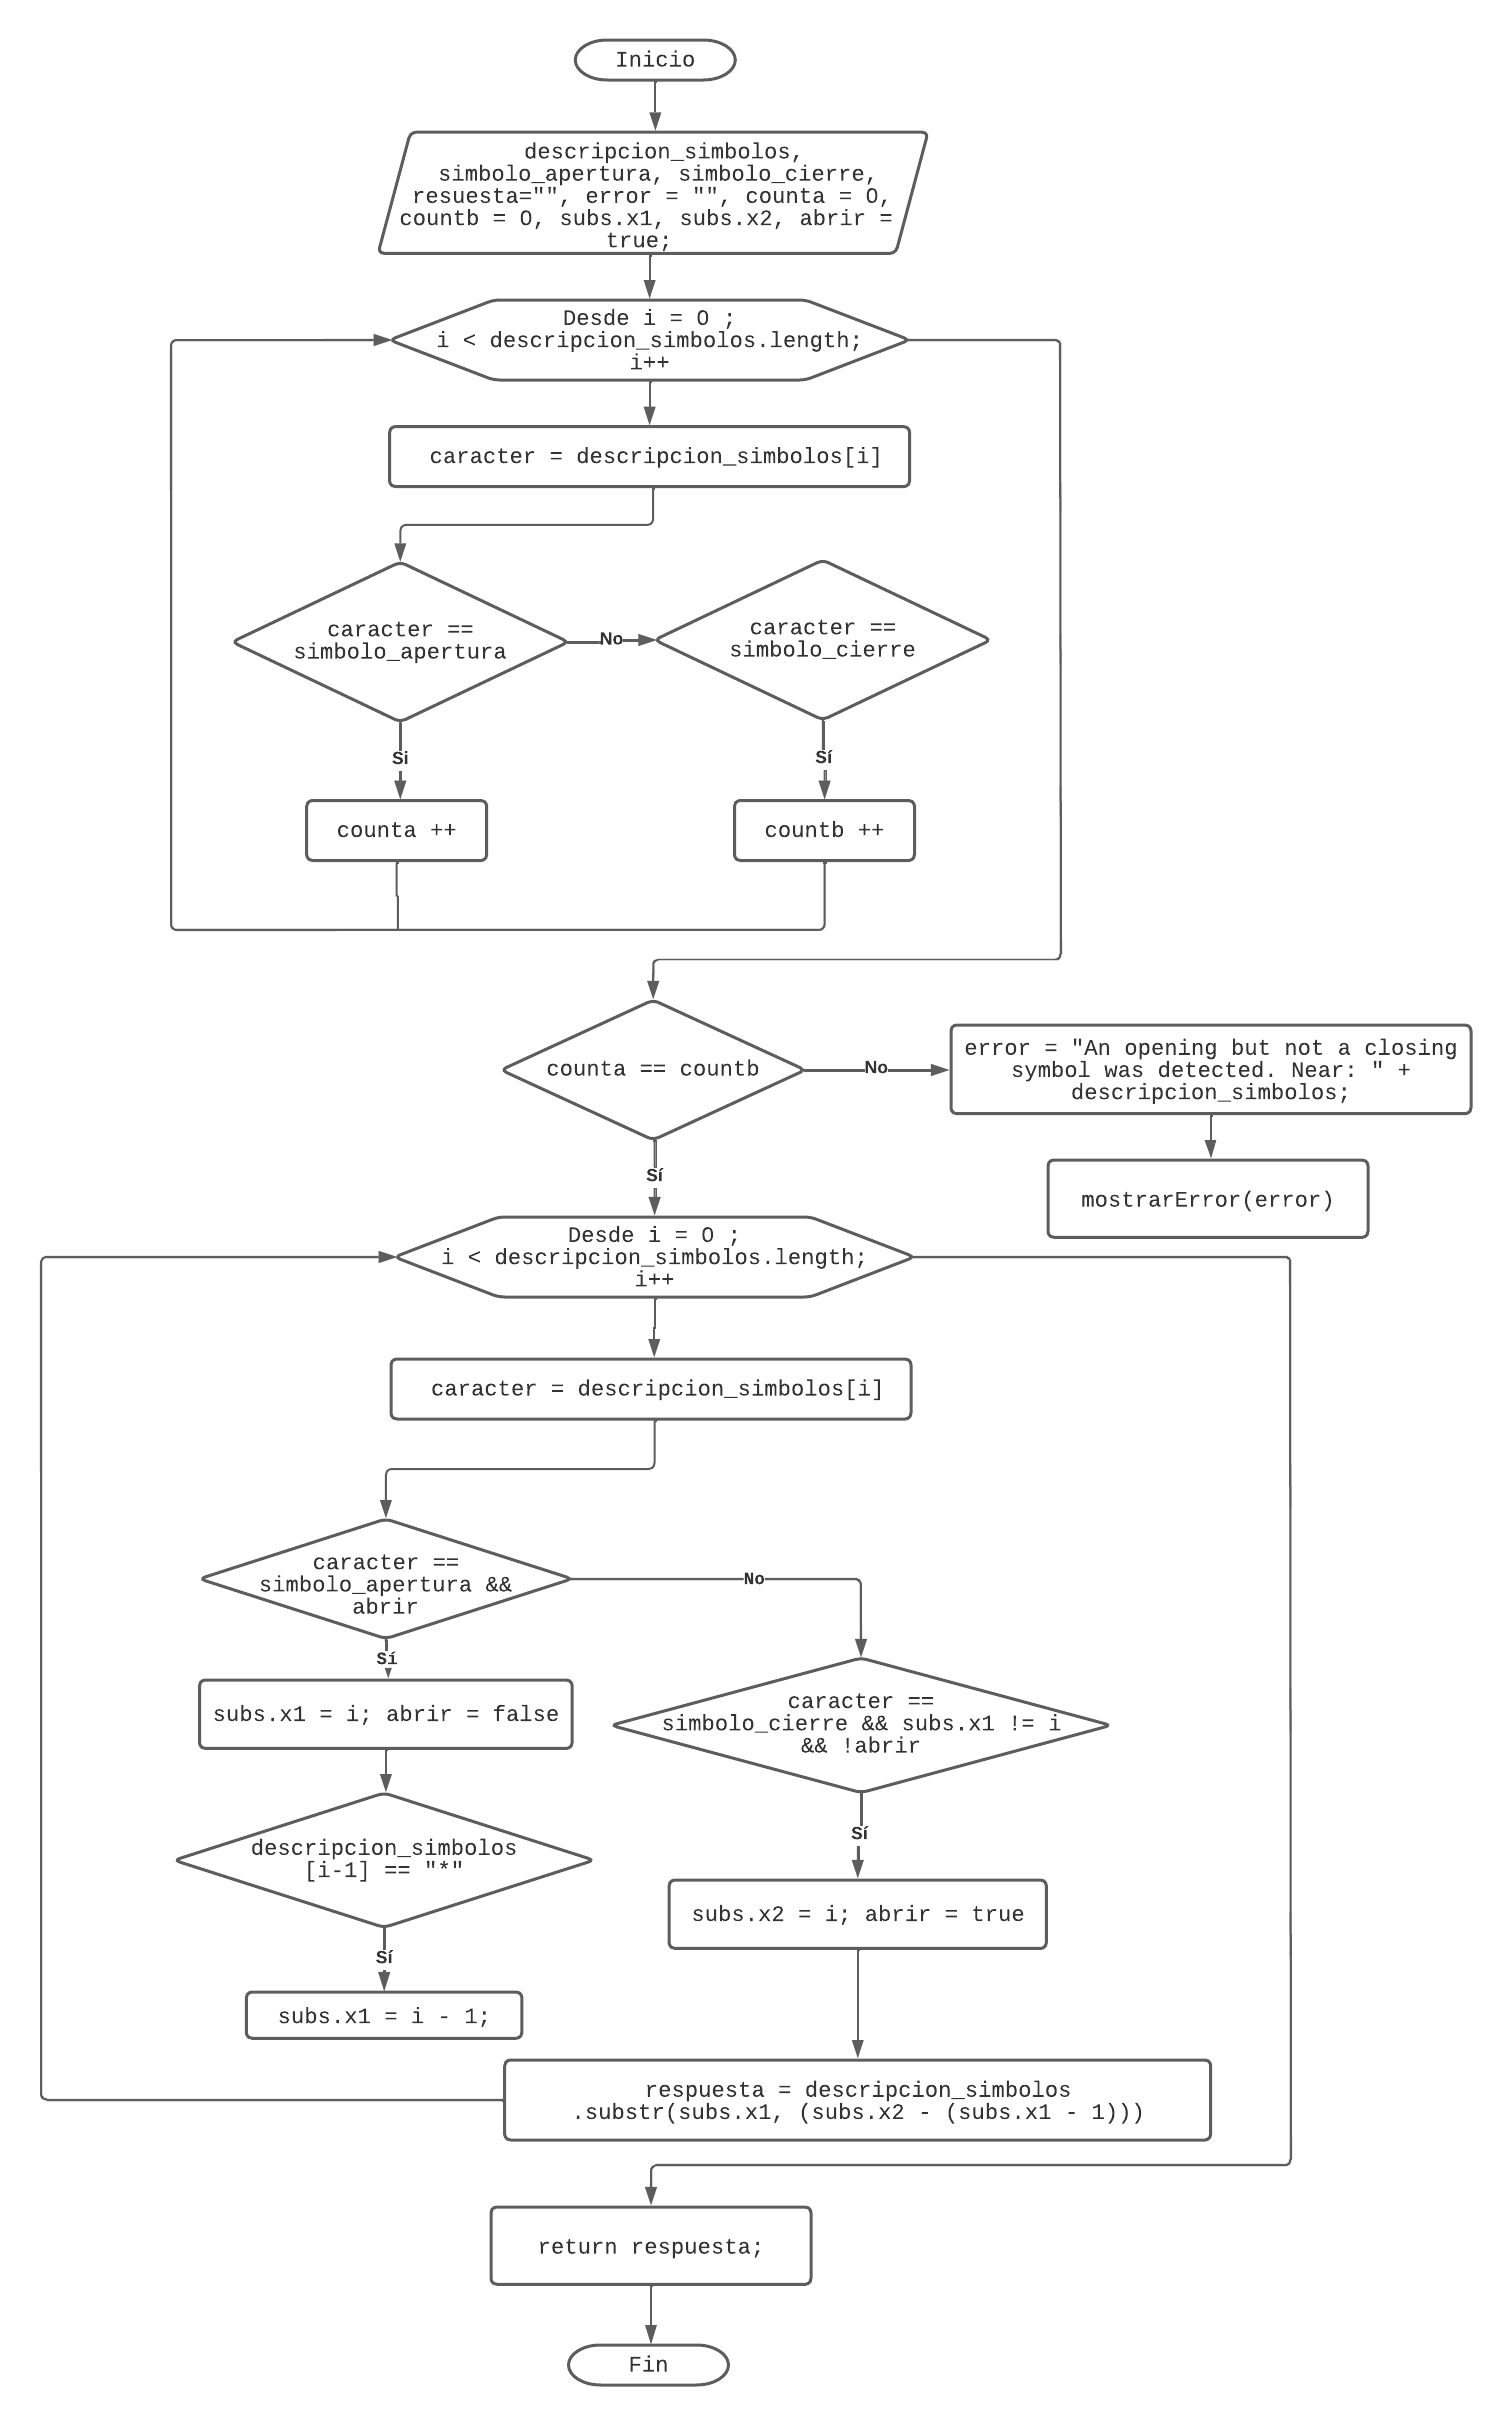
\includegraphics[width=11cm]{img/algoritmoerror.png}
	\label{fig:algoritmoerror}
	\textbf{\\ \\ ELABORADO: DÚVAL CARVAJAL SUÁREZ}
\end{figure} 

\section{Generación de código}

En la siguiente fase se desarrollaron las funciones y todos los métodos que fueron necesarios para que la librería funcione correctamente. A continuación se observan todas las variables que fueron necesarias para que todo funcione de manera correcta.

\lstinputlisting[language=java]{codigo/variables.js}

En el siguiente bloque de código se observa la función que permite acumular los mensajes de error que pueden ocurrir al momento de interpretar las descripciones de los casos de uso. 

\lstinputlisting[language=java]{codigo/notificaciones.js}

En el siguiente bloque de código se observa una de las funciones principales para detectar los símbolos de apertura y cierre, con el objetivo de utilizar una sola función que permita identificar los símbolos que necesariamente deben ser con apertura y cierre. 

\lstinputlisting[language=java]{codigo/detectarsimbolos.js}

\section{Ejecución de pruebas}

Para la ejecución de las pruebas, se analizaron los textos que se recopilaron en la fase inicial. Lo que se realizo fue ingresar los textos de prueba y obtener como resultado lo esperado por la librería.

\section{Evaluación con sistemas de información}
